\documentclass[11pt]{article}

\usepackage[margin=1in]{geometry}
\usepackage[T1]{fontenc}
\usepackage[utf8]{inputenc}
\usepackage{lmodern}
\usepackage{microtype}
\usepackage{amsmath,amssymb,amsthm,mathtools}
\usepackage{booktabs}
\usepackage{longtable}
\usepackage{tabularx}
\usepackage{array}
\usepackage{float}
\usepackage{enumitem}
\usepackage{fancyvrb}
\usepackage{xcolor}
\usepackage{hyperref}
\usepackage{xurl}
\usepackage{xspace}
\usepackage{tikz}
\usetikzlibrary{arrows.meta,positioning,fit,calc,shapes.geometric}

\hypersetup{
  colorlinks=true,
  linkcolor=blue!50!black,
  urlcolor=blue!50!black,
  citecolor=blue!50!black,
  pdftitle={cTEE: Cryptographic Trusted Execution Envelopes - Private Workspaces and Protected Agency on Untrusted Compute},
  pdfauthor={cTEE}
}

\newtheorem{definition}{Definition}
\newtheorem{theorem}{Theorem}
\newtheorem{lemma}{Lemma}
\newtheorem{proposition}{Proposition}
\newtheorem{corollary}{Corollary}
\newtheorem{assumption}{Assumption}
\newtheorem{invariant}{Invariant}

\newcommand{\ctee}{\textnormal{\textsc{cTEE}}}
\newcommand{\pwc}{\textnormal{\textsc{PrivateWorkspace}}}
\newcommand{\roletext}[1]{\textnormal{\textsc{#1}}\xspace}
\newcommand{\node}{\ifmmode\mathsf{Node}\else\roletext{Node}\fi}
\newcommand{\guard}{\ifmmode\mathsf{Guardian}\else\roletext{Guardian}\fi}
\newcommand{\user}{\ifmmode\mathsf{User}\else\roletext{User}\fi}
\newcommand{\ag}{\ifmmode\mathsf{StateLog}\else\roletext{StateLog}\fi}
\newcommand{\store}{\ifmmode\mathsf{BlobStore}\else\roletext{BlobStore}\fi}
\newcommand{\aead}{\ensuremath{\mathsf{AEAD}}}
\newcommand{\enc}{\ensuremath{\mathsf{Enc}}}
\newcommand{\dec}{\ensuremath{\mathsf{Dec}}}
\newcommand{\commit}{\ensuremath{\mathsf{Com}}}
\newcommand{\hash}{\ensuremath{\mathsf{H}}}
\newcommand{\sig}{\ensuremath{\mathsf{Sig}}}
\newcommand{\verify}{\ensuremath{\mathsf{Verify}}}
\newcommand{\leak}{\mathcal{L}}
\newcommand{\view}{\mathsf{View}}
\newcommand{\adv}{\mathcal{A}}
\newcommand{\negl}{\mathsf{negl}}
\newcommand{\code}[1]{\texttt{#1}}
\newcommand{\term}[1]{\textit{#1}}
\newcommand{\vect}[1]{\mathbf{#1}}

\definecolor{artifactframe}{RGB}{52,73,94}
\definecolor{artifactfill}{RGB}{246,249,252}
\definecolor{artifacttitlefill}{RGB}{232,239,245}
\newcommand{\doctrinebox}[1]{%
\medskip
\noindent\begingroup
\setlength{\fboxsep}{8pt}%
\fcolorbox{artifactframe}{artifactfill}{\parbox{\dimexpr\linewidth-2\fboxsep-2\fboxrule}{#1}}%
\endgroup
\medskip
}

\newenvironment{protocol}[1]{%
  \medskip
  \noindent\textbf{Protocol. #1}\par\smallskip
  \begingroup
}{%
  \par\endgroup
  \medskip
}

\setlength{\emergencystretch}{3em}

\title{\ctee{}: Cryptographic Trusted Execution Envelopes\\[0.35em]
\large Private Workspaces and Protected Agency on Untrusted Compute}
\author{cTEE Yellow Paper}
\date{June 1, 2026}

\begin{document}
\maketitle

\begin{abstract}
Modern agent harnesses increasingly need persistent remote compute: rented GPUs,
hosted workers, decentralized compute nodes, service marketplaces, and
always-on cloud workspaces. The standard deployment model gives the remote node
a plaintext workspace and then asks containers, VMs, process sandboxes, or boot
measurements to keep a root-level provider from reading it. That model is
wrong for high-value agent state. A provider with root can usually inspect
files, logs, process memory, prompts, tool inputs, and GPU-visible buffers.

This paper introduces \ctee{}s, Cryptographic Trusted Execution Envelopes, as a
software systems pattern for private autonomous agents on untrusted compute.
A \ctee{} is not a hardware TEE and does not claim to hide arbitrary plaintext
memory from root. Its central invariant is stricter: protected workspace state
is not given to the untrusted node as normal plaintext in the first place.
The user-facing primitive is an \term{Open Private Workspace}; the node-facing
primitive is a cryptographic execution envelope over encrypted workspace
objects, public trunks, sealed private heads, commitments, receipts, leakage
profiles, declassification gates, and capability exits.
A \ctee{} can be bound to any private agent harness, enterprise runner,
DePIN network, worker runtime, or service marketplace that can provide an
authority view, execution boundary, state log, artifact store, and optional
settlement layer.

The paper contributes: (1) a formal no-plaintext-custody model for private
agent workspaces; (2) a concrete object and protocol suite including
\code{PrivateWorkspaceNode}, \code{PrivateWorkspaceCapsule}, \code{AlphaSeal},
\code{AutonomyLease}, \code{DeclassificationReceipt}, and
\code{PrivateInferenceReceipt}; (3) a compositional security treatment for
privacy, authority, restore validity, and receipt binding; and (4) a practical
default high-throughput execution strategy, Candidate-Lattice Private Decoding,
that keeps ordinary GPU token speed for public model work while moving private
selection, private policy, or private strategy heads outside the untrusted
node. It also defines Plaintext-Free Runtime Mounting, including
Plaintext-Free Model Mounting, as the runtime interface that exposes private
workspaces to runtimes as public/redacted content, encrypted refs, private
handles, and capability exits rather than provider-readable plaintext.
We also state a negative result: arbitrary full-speed private LLM
inference on a single root-controlled consumer GPU is not obtained by software
wrapping alone. Useful privacy requires either no plaintext custody, trusted
hardware, a trusted or threshold guardian, or cryptographic evaluation with its
own overhead. \ctee{}s make that tradeoff explicit and productizable.
\end{abstract}

\tableofcontents
\newpage

\section{Motivation}

Private autonomous agents need compute that can stay awake. A developer may
want to rent a cheap RTX 3090 node to run a persistent agent harness. A quant
user may want the node to fetch market data, run backtests, simulate models,
draft reports, and propose trades while the user's laptop is asleep. An
enterprise may want a service marketplace to spin up decentralized compute for
a private outcome. In each case the economic reason to use the node is clear:
GPU time is cheaper or more available away from the user's local machine.

The privacy problem is equally clear. If the remote workspace contains:

\begin{Verbatim}[fontsize=\small]
/workspace/strategy.py
/workspace/signals.py
/workspace/risk.py
/workspace/config.yaml
\end{Verbatim}

\noindent as ordinary plaintext, a root-level provider can likely copy the
files, snapshot the disk, trace the process, inspect logs, and watch prompts.
An encrypted disk image helps at rest, but once the guest mounts the volume and
the agent reads the strategy, the provider-controlled host can often observe
the plaintext through some layer of the system. A container boundary is not a
privacy theorem.

\doctrinebox{\textbf{cTEE doctrine.} The node can compute against the
workspace, but it should not custody workspace secrets.}

\subsection{Why This Is Not Encryption at Rest}

Encryption at rest protects stored bytes until a program decrypts them. It
does not, by itself, protect the plaintext once the remote workspace mounts
the volume, prompts a model, runs a tool, writes a log, caches a result, or
places intermediate values in provider-visible memory.

\ctee{} changes the routing contract. Protected state is not mounted,
prompted, logged, cached, traced, or executed as provider-readable plaintext on
the untrusted node. The node receives public trunks, redacted projections,
encrypted refs, commitments, candidate lattices, and receipts. Plaintext views
and declassification decisions live in the user's authority view.

\ctee{}s are proposed as the missing middle between two bad extremes:

\begin{enumerate}[leftmargin=1.5em]
\item \textbf{Plain cloud workspace.} Fast and useful, but the provider can
read the secrets.
\item \textbf{Pure cryptographic private inference.} Stronger privacy, but
today usually too slow or too narrow for arbitrary agentic LLM work.
\end{enumerate}

\ctee{}s keep the useful fast path by splitting work into public or redacted
trunks that can run on the rented GPU, and private heads that remain sealed,
masked, secret-shared, guardian-mediated, or locally evaluated.

\section{Contributions}

This yellow paper defines \ctee{}s as a systems primitive, not a new
cryptographic primitive. Its technical contribution is a custody discipline for
private agency: a way to transform many secret-bearing agent tasks into public
candidate expansion, private choice, receipted declassification, and
capability-bounded action.

\begin{enumerate}[leftmargin=1.5em]
\item \textbf{No-Plaintext-Custody Security.} We formalize the property that an
untrusted node's view is simulatable from declared leakage, public trunks,
encrypted refs, commitments, and receipts.
\item \textbf{Private Workspace Object Model.} We define the objects needed to
make ``Open Private Workspace'' real: encrypted workspace objects, private
workspace capsules, sealed private heads, autonomy leases, declassification
receipts, and capability exits.
\item \textbf{Split-State Agent Automaton.} We model agent execution as a state
machine whose state is partitioned into public, redacted, sealed, guardian, and
action-authority components.
\item \textbf{Custody Type System.} We define a small type discipline for
plaintext custody. Values are typed as public, redacted, sealed, guardian-only,
cryptographic-operator, capability-only, or never-remote-plaintext, and runtime
mounts must type-check before node exposure.
\item \textbf{Proof-Carrying Workspace.} We define a verifiable custody proof
that binds sensitivity labels, mount graph, operator routing, receipts, leakage
budget, and state roots. A result can carry evidence that protected values did
not enter node plaintext custody.
\item \textbf{Private Agency Transform.} We formalize the reduction from
private inference to public proposal plus private selection for
candidate-selection-reducible tasks. This is the theorem-shaped reason cTEEs
can preserve node-side token speed for useful private agency without claiming
arbitrary private LLM inference.
\item \textbf{Candidate Coverage Frontier.} We show that zero online
private-selection leakage can be purchased with public overgeneration in
proportion to candidate redundancy mass. When acceptable complete traces retain
non-negligible public probability mass, the trace budget is depth-independent;
when that mass decays exponentially, cTEE must route away from CLPD/CLE.
\item \textbf{Counterfactual Lattice Execution.} We introduce a high-assurance
CLPD schedule in which the node expands a committed lattice of plausible
futures before learning any private selection. The private path is hidden inside
counterfactual public work, replacing step-by-step selection leakage with final
declassification leakage at the cost of extra public token volume.
\item \textbf{External Model API Boundary.} We distinguish cTEE
no-plaintext-custody from provider trust. A third-party model API that receives
sensitive plaintext is outside the base cTEE custody claim unless the payload is
public, redacted, declassified, or protected by a separately verifiable
private-compute interface.
\item \textbf{AlphaSeal.} We define a reusable sealed-private-head pattern for
quant strategies and other high-value decision logic.
\item \textbf{Candidate-Lattice Private Decoding.} We introduce the default
\ctee{} protected-agency strategy: an untrusted GPU generates public candidate
lattices at normal speed while a private head selects, filters, or reranks
without revealing the private policy.
\item \textbf{Plaintext-Free Runtime Mounting.} We define the runtime mount
boundary that presents private workspaces to tools, files, shells, model
servers, and model calls as public trunks, redacted projections, encrypted
refs, private-function handles, declassification requests, and capability exits
rather than plaintext private files or prompts. \code{PlaintextFreeModelMount}
is the model-facing specialization.
\item \textbf{Cryptographic Operator Plane.} We define the internal operator
plane that routes protected subcomputations to FHE, MPC, garbled circuits,
ORAM, local guardian, or threshold guardian paths. The default second logical
party is the user's existing authority surface, not a new managed committee.
\item \textbf{Deterrence and Detection.} We specify synthetic canaries,
provider-bound watermarks, honeytokens, leak scans, replay checks, and receipts
as attribution and dispute evidence. These mechanisms do not make plaintext
safe; they make abuse more detectable.
\item \textbf{Receipt and Restore Composition.} We specify how receipts,
commitments, encrypted blobs, and state roots make private agent work
auditable and restorable without exposing plaintext to the compute provider.
\end{enumerate}

\subsection{Security Claims and Non-Claims}

\begin{tabularx}{\linewidth}{p{0.22\linewidth}X}
\toprule
\textbf{Claims} &
The node does not receive plaintext custody of protected workspace objects.
Private objects are encrypted, committed, redacted, guardian-mediated, or
handled through explicit capability exits. External effects require authority
and receipts. Restore/import is state-root and policy checked. \\
\midrule
\textbf{Non-claims} &
\ctee{} does not claim arbitrary full-speed private LLM inference by software
wrapping alone. It does not eliminate all metadata, timing, size, schedule, or
selection leakage. It does not protect a workspace that the user explicitly
mounts on the rented node as ordinary plaintext. It does not turn a
third-party model API that receives sensitive plaintext into a
no-plaintext-custody system. \\
\bottomrule
\end{tabularx}

\subsection{External Model API Boundary}

The cTEE privacy claim is a custody claim. It is strongest when the user,
service, or organization controls the compute substrate: local GPU, rented GPU,
customer VPC node, DePIN node, or another venue where protected state can stay
outside provider-readable plaintext custody.

If sensitive plaintext is sent to a third-party model API, the run leaves the
base cTEE no-plaintext-custody model for that data and enters a provider-trust
model. Contractual no-training terms, retention controls, enterprise privacy
policies, and legal commitments may be useful, but they are not the same claim
as never giving the provider sensitive plaintext.

\begin{itemize}[leftmargin=1.5em]
\item \textbf{Private-native.} Sensitive plaintext does not leave cTEE custody.
Models run locally, on rented/self-hosted compute, in customer-controlled
venues, or through private operators.
\item \textbf{Redacted-API.} A third-party API receives only public data,
redacted projections, synthetic/counterfactual candidates, or explicitly
declassified payloads.
\item \textbf{Provider-trust.} A third-party API may receive sensitive plaintext
under contract, policy, retention promises, attestation, or other trust claims.
This is outside base cTEE no-plaintext-custody unless the API exposes a
separately verifiable private-compute interface.
\item \textbf{Unsafe.} Private data enters untrusted plaintext custody without
explicit declassification or accepted provider-trust policy.
\end{itemize}

This distinction is economic as well as cryptographic. If a user rents a GPU
node, extra candidate or counterfactual generation consumes leased GPU time and
wall-clock latency. If the same strategy is implemented through third-party API
tokens, extra private-preserving branches may burn API budget and may also
expose plaintext unless the API path is public, redacted, declassified, or
separately protected.

\section{System Model}

\subsection{Participants}

A \ctee{} deployment has the following roles:

\begin{description}[leftmargin=1.8em]
\item[\user.] The human, organization, or local client that owns private
workspace state.
\item[\node.] The untrusted rented, hosted, provider, or DePIN compute node. It
may have a GPU and may run an agent harness. It is assumed provider-rooted.
\item[\guard.] A trusted, threshold, or policy-controlled authority path that
can hold keys, evaluate narrow private heads, approve declassification, or sign
capability exits. This may be a browser/device, mobile signer, enterprise key
service, MPC committee, HSM, or confidential environment.
\item[\ag.] The append-only or operation-backed state log that records
workspace refs, commits, receipts, state roots, policy hashes, and restore
metadata. The state log is the canonical meaning layer for sealed objects,
not the place where all payload bytes must live.
\item[\store.] The blob storage plane. It holds encrypted payload bytes, sealed
archives, traces, checkpoints, public datasets, and large artifacts. It does
not define what those bytes mean.
\end{description}

\subsection{Guardian as Authority View}

The guardian is a formal role, not necessarily a separate machine the user must
operate. In the common product path, the guardian is the user's existing
authority view:

\begin{itemize}[leftmargin=1.5em]
\item an authenticated browser instance that renders decrypted private files;
\item a desktop agent harness or CLI holding an interactive workspace session;
\item an authority plane or signing path backed by passkeys, hardware keys,
mobile approval, policy services, or threshold custody;
\item a customer VPC service, enterprise HSM, or policy service for teams;
\item a small always-on authority worker for unattended \code{AutonomyLease}
checks.
\end{itemize}

Thus \ctee{} does not require a second runtime beside the rented GPU node. It
separates compute custody from view/sign/declassify custody. The user already
needs some surface that can decrypt and display private workspace content; the
guardian names that surface when it also evaluates private heads, applies
declassification policy, or approves capability exits.

\doctrinebox{\textbf{Authority-view doctrine.} The rented node is the compute
workspace. The browser, authority plane, local harness, CLI, or threshold
authority is the private view and signing membrane.}

\subsection{Architecture at a Glance}

\begin{figure}[H]
\centering
\small
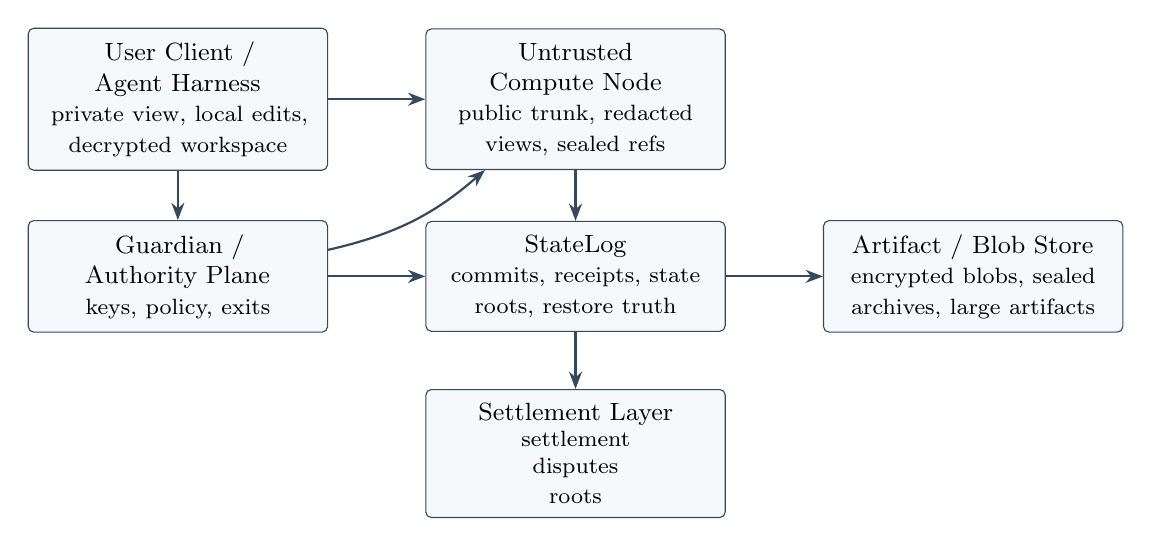
\begin{tikzpicture}[
  box/.style={
    draw=artifactframe,
    fill=artifactfill,
    rounded corners=2pt,
    align=center,
    text width=3.45cm,
    minimum height=1.25cm,
    inner sep=5pt
  },
  arrow/.style={-{Stealth[length=2.2mm]}, thick, draw=artifactframe},
  every node/.style={font=\small}
]
\node[box] (userbox) at (0,0)
  {User Client /\\Agent Harness\\
   \footnotesize private view, local edits, decrypted workspace};
\node[box] (guardbox) at (0,-2.25)
  {Guardian /\\Authority Plane\\
   \footnotesize keys, policy, exits};
\node[box] (nodebox) at (5.05,0)
  {Untrusted\\Compute Node\\
   \footnotesize public trunk, redacted views, sealed refs};
\node[box] (agbox) at (5.05,-2.25)
  {StateLog\\
   \footnotesize commits, receipts, state roots, restore truth};
\node[box] (storebox) at (10.1,-2.25)
  {Artifact / Blob Store\\
   \footnotesize encrypted blobs, sealed archives, large artifacts};
\node[box] (l1box) at (5.05,-4.5)
  {Settlement Layer\\
   \footnotesize settlement\\disputes\\roots};

\draw[arrow] (userbox) -- (nodebox);
\draw[arrow] (userbox) -- (guardbox);
\draw[arrow] (nodebox) -- (agbox);
\draw[arrow] (guardbox) -- (agbox);
\draw[arrow] (agbox) -- (storebox);
\draw[arrow] (agbox) -- (l1box);
\draw[arrow] (guardbox) to[bend right=14] (nodebox);
\end{tikzpicture}
\caption{\ctee{} splits plaintext custody from compute custody. The rented
node receives useful work but not protected workspace plaintext. The state log
records meaning, receipts, policy, and restore truth; artifact stores hold
bytes; public settlement is sparse and trigger-based.}
\end{figure}

\subsection{Reference Bindings}

\ctee{} is ecosystem-neutral. A deployment binds the generic roles above to
its own runtime, authority, state, storage, marketplace, and settlement
components. The protocol does not require Agentgres, wallet.network, IOI L1,
or any particular marketplace. Those names are one concrete IOI binding:

{\small
\begin{description}[leftmargin=2.3em,style=nextline]
\item[Guardian / authority view.] Authenticated browser, local Autopilot, CLI
signer, wallet.network-backed authority.
\item[Authority plane.] wallet.network for grants, scopes, revocation, secrets,
payments, and decryption leases.
\item[Execution boundary.] IOI daemon for tool/model execution, sensitive-exit
trapping, and runtime mount enforcement.
\item[Plaintext-Free Runtime Mount.] Default Harness Profile cTEE mount inside
the daemon.
\item[StateLog.] Agentgres for admitted refs, receipts, state roots, policy
hashes, and restore truth.
\item[Artifact / blob store.] Agentgres Artifact Plane plus storage backends
such as local disk, S3, Filecoin, CAS/IPFS, and object stores.
\item[Settlement layer.] IOI L1 or compatible app chains for public, economic,
dispute, or cross-domain commitments only when triggered.
\item[Worker marketplace.] aiagent.xyz for discovery, manifests, benchmarks,
reputation, and licensing. It advertises capabilities; it does not grant
capabilities.
\item[Outcome marketplace.] sas.xyz for service ordering, delivery, acceptance,
dispute, remediation, and settlement profile. Authority still exits through
the daemon and wallet.network.
\end{description}
}

\doctrinebox{\textbf{Binding doctrine.} cTEE defines the privacy and custody
envelope. A concrete stack binds that envelope to an authority plane, execution
boundary, state log, artifact store, and settlement layer. Marketplaces may
advertise or contract for capabilities and outcomes, but they do not grant
capabilities.}

\subsection{Adversary}

The adversary controls \node. It can:

\begin{itemize}[leftmargin=1.5em]
\item read node files, logs, environment variables, process memory, and normal
GPU-visible buffers;
\item snapshot disks and RAM;
\item observe network timing, job sizes, model family, public datasets, and
resource usage;
\item delay, abort, replay, fork, or equivocate about node execution;
\item return invalid outputs or try to get paid for fake work.
\end{itemize}

The adversary does not break standard cryptographic assumptions, does not
compromise \guard unless the chosen guardian threshold permits it, and does not
force the user to explicitly declassify protected state. Hardware TEEs may be
used as an optional strengthening layer, but the base \ctee{} model does not
depend on them.

\subsection{State Partition}

Let an agent workspace state \(S\) be partitioned as:

\[
S = S_{\mathsf{pub}} \parallel S_{\mathsf{red}} \parallel
    S_{\mathsf{seal}} \parallel S_{\mathsf{guard}} \parallel
    S_{\mathsf{auth}}.
\]

\begin{itemize}[leftmargin=1.5em]
\item \(S_{\mathsf{pub}}\): public files, public model weights, public data,
public tools.
\item \(S_{\mathsf{red}}\): redacted summaries, public stubs, sanitized
prompts, padded labels.
\item \(S_{\mathsf{seal}}\): encrypted private workspace objects, sealed
strategy heads, encrypted archives, commitments.
\item \(S_{\mathsf{guard}}\): state available only to \guard or a threshold
committee, such as key shares, private coefficients, private selectors, or
declassification policy.
\item \(S_{\mathsf{auth}}\): action authority, including signing keys, broker
capability scopes, payment authority, and revocation state.
\end{itemize}

The core \ctee{} invariant is:

\[
\view_{\node} \subseteq
f(S_{\mathsf{pub}}, S_{\mathsf{red}}, \enc(S_{\mathsf{seal}}),
  \commit(S_{\mathsf{guard}}), \leak)
\]

\noindent for declared leakage \(\leak\). The node's view must not require
plaintext \(S_{\mathsf{seal}}\), \(S_{\mathsf{guard}}\), or \(S_{\mathsf{auth}}\).

\section{Cryptographic Preliminaries}

\subsection{Authenticated Encryption}

Workspace objects are encrypted with an authenticated encryption scheme:

\[
C \leftarrow \aead.\enc_K(N, A, M),
\qquad
M \leftarrow \aead.\dec_K(N, A, C).
\]

\noindent The associated data \(A\) should bind workspace identity, object id,
schema version, policy hash, content role, state root, and expected parent
head. This prevents ciphertext transplant across workspaces or policy epochs.

\subsection{Commitments}

A commitment scheme provides hiding and binding commitments. For scalar or
vector values, a Pedersen-style commitment has the form:

\[
C = rH + \sum_i v_i G_i,
\]

\noindent where \(r\) is a random blinding factor and \(G_i,H\) are independent
generators. It is additively homomorphic:

\[
C(\vect{v}, r) + C(\vect{w}, s) =
C(\vect{v} + \vect{w}, r+s).
\]

This is useful in \ctee{}s for private scores, private risk budgets, aggregate
usage, masked rankings, and proof-carrying receipts. The commitment is not a
substitute for encryption; it is a public binding to a private value.

\subsection{Homomorphic Encryption, MPC, Garbled Circuits, and ORAM}

Fully homomorphic encryption (FHE) evaluates circuits over ciphertexts.
Approximate arithmetic schemes such as CKKS are relevant for vector and neural
arithmetic, but have cost, precision, and circuit-depth constraints. Secure
multi-party computation (MPC) distributes computation across parties such that
privacy holds against a bounded collusion threshold. Garbled circuits are often
effective for boolean or branching logic. Oblivious RAM (ORAM) hides access
patterns at a bandwidth and complexity cost.

\ctee{}s treat these as operator families:

\[
\mathsf{Op} \in
\{\mathsf{Public}, \mathsf{Redacted}, \mathsf{FHE}, \mathsf{MPC},
\mathsf{GC}, \mathsf{ORAM}, \mathsf{Guardian}, \mathsf{TEE}\}.
\]

The envelope chooses the cheapest operator family that satisfies the sensitivity
policy. It does not require every operation to be FHE.

\subsection{Receipts}

A receipt is a signed or hash-addressed statement that binds:

\[
R = \hash(\mathsf{actor}, \mathsf{operation}, \mathsf{inputs},
\mathsf{outputs}, \mathsf{policy}, \mathsf{authority}, \mathsf{stateRoot},
\mathsf{time}).
\]

Receipts let the system prove that an operation occurred under a policy without
revealing protected payloads. A receipt may include commitments instead of
plaintext outputs.

\section{cTEE Syntax}

A \ctee{} scheme is a tuple of algorithms:

\[
\Pi_{\ctee} =
(\mathsf{Setup}, \mathsf{Open}, \mathsf{Seal}, \mathsf{Patch},
\mathsf{Compile}, \mathsf{Eval}, \mathsf{Declassify},
\mathsf{Exit}, \mathsf{Commit}, \mathsf{Restore}).
\]

\begin{description}[leftmargin=1.8em]
\item[\(\mathsf{Setup}(1^\lambda)\).] Generates system parameters, encryption
profiles, commitment parameters, supported operator families, and receipt
schemas.
\item[\(\mathsf{Open}(\user, P)\).] Opens a private workspace under policy
\(P\). The user sees ordinary files and folders; the node sees only permitted
views.
\item[\(\mathsf{Seal}(W, M, role)\).] Encrypts a workspace object \(M\) into a
sealed object \(C\) with role metadata, state roots, and policy-bound AAD.
\item[\(\mathsf{Patch}(W, \Delta)\).] Converts a user edit into an encrypted
patch, a public trunk patch, or a redacted projection update.
\item[\(\mathsf{Compile}(task, P)\).] Compiles a task into a
\code{PrivateWorkspaceCapsule}: visible context, protected refs, allowed remote
ops, forbidden plaintext classes, leakage profile, and required receipts.
\item[\(\mathsf{Eval}(\node, capsule)\).] Executes public, redacted, masked,
encrypted, or guardian-mediated operations and emits commitments and receipts.
\item[\(\mathsf{Declassify}(Y, P, grant)\).] Converts a protected output into a
visible result or denies/escalates it.
\item[\(\mathsf{Exit}(a, P, grant)\).] Performs an external action through a
capability exit, such as broker order signing, API write, email send, or
deployment.
\item[\(\mathsf{Commit}(R)\).] Records refs, receipts, commitments, and state
roots in \ag.
\item[\(\mathsf{ProveCustody}(trace, P)\).] Produces a
\code{CustodyProof} from the sensitivity manifest, custody derivation, mount
graph, receipts, leakage budget, and state roots.
\item[\(\mathsf{VerifyCustody}(\pi, P)\).] Verifies that a custody proof
\(\pi\) is consistent with policy, receipts, and state roots.
\item[\(\mathsf{Restore}(archive, P)\).] Rehydrates workspace state after
authority checks, hash verification, decryption, and state-root validation.
\end{description}

\section{Leakage-Typed cTEE-IR}

The compiler is the enforcement point. A \ctee{} implementation should not rely
on operator authors to remember which data may touch an untrusted node. It
should compile agent work into a leakage-typed intermediate representation
whose typing rules reject accidental plaintext custody before execution.

\subsection{Sensitivity Lattice}

Let sensitivity labels form a partial order:

\[
\mathsf{public} \sqsubset
\mathsf{redacted} \sqsubset
\mathsf{sealed} \sqsubset
\mathsf{guardian} \sqsubset
\mathsf{authority}.
\]

The order is not a disclosure permission. It is a custody boundary. Public and
approved redacted values may be materialized on \node. Sealed values may appear
only as ciphertexts, commitments, shares, or handles. Guardian values may be
materialized only inside \guard or a threshold policy path. Authority values may
never be handed to \node; they can only be exercised through capability exits.

Each expression has a type and label:

\[
\Gamma \vdash e : \tau^{\ell},
\qquad
\ell \in
\{\mathsf{public}, \mathsf{redacted}, \mathsf{sealed},
\mathsf{guardian}, \mathsf{authority}\}.
\]

The label of a derived expression is at least the join of its dependencies:

\[
\ell(e_1 \circ e_2) \sqsupseteq \ell(e_1) \sqcup \ell(e_2).
\]

\subsection{Custody Kinds}

Sensitivity labels say what a value is. Custody kinds say where its plaintext
may ever be materialized:

\[
\Gamma \vdash e : \tau^{\ell}@\kappa.
\]

\noindent The base custody kinds are:

\begin{description}[leftmargin=2.4em]
\item[\(\mathsf{Public}\).] Plaintext may be materialized on the node.
\item[\(\mathsf{Redacted}\).] A policy-approved projection may be materialized
on the node, but the source value may not.
\item[\(\mathsf{Sealed}\).] The node may hold ciphertexts, commitments,
shares, or opaque refs only.
\item[\(\mathsf{GuardianOnly}\).] Plaintext may be materialized only inside the
authority view, local client, browser, mobile guardian, or threshold path.
\item[\(\mathsf{CryptoOperator}\).] The value may participate in an approved
FHE, MPC, garbled-circuit, ORAM, local-guardian, or threshold operator.
\item[\(\mathsf{CapabilityOnly}\).] The value is authority, not data. The node
may request an action, but cannot read the credential or grant material.
\item[\(\mathsf{NeverRemotePlaintext}\).] The value has no valid node-plaintext
projection under the current policy.
\end{description}

A remote plan type-checks only when every edge into the node has a custody kind
that admits the planned node-visible representation. This makes plaintext
custody a property of the compiled graph, not a convention remembered by tool
authors.

\subsection{Remote Admissibility}

An operator \(op\) may be scheduled on \node only if the compiler can derive:

\[
\Gamma, P \vdash op(e_1,\ldots,e_n)
\Downarrow_{\node}
(y, R, \leak_{op})
\]

\noindent subject to one of the following admissibility rules:

\begin{enumerate}[leftmargin=1.5em]
\item \textbf{Plain remote rule.} Every input label is
\(\mathsf{public}\) or policy-approved \(\mathsf{redacted}\), and the output is
not more sensitive than policy permits.
\item \textbf{Cryptographic remote rule.} Any sealed input is represented on
\node only as FHE ciphertext, MPC share, garbled-circuit wire label, ORAM
handle, encrypted blob ref, or commitment. The operator family must match the
representation.
\item \textbf{Guardian-mediated rule.} The node may issue a bounded query to
\guard and receive only an approved response class: selection bit, masked
score, redacted critique, encrypted result, or declassification denial.
\item \textbf{Capability-exit rule.} Authority-labeled values cannot be read.
The node may propose an action; \guard, the authority plane, or the execution
boundary decides whether to execute it through a scoped capability exit.
\end{enumerate}

If no rule applies, the compiler must reject the remote plan or repartition the
task. This is the practical meaning of no-plaintext custody.

\subsection{Receipt-Carrying Types}

Remote execution returns values with receipt obligations:

\[
\Gamma, P \vdash op : \tau_1^{\ell_1} \times \cdots \times \tau_n^{\ell_n}
\to \tau_o^{\ell_o} \; [\mathcal{R}, \leak_{op}].
\]

\noindent Here \(\mathcal{R}\) is the set of required receipts, for example:

\begin{itemize}[leftmargin=1.5em]
\item \code{PrivateInferenceReceipt};
\item \code{PrivateOperatorReceipt};
\item \code{CounterfactualLatticeReceipt};
\item \code{ArtifactRecordedReceipt};
\item \code{DeclassificationReceipt};
\item \code{CapabilityExitReceipt}.
\end{itemize}

A value whose receipt obligations are unsatisfied cannot be committed as
admitted workspace truth.

\subsection{Compiler Invariant}

\begin{invariant}[No Plaintext by Construction]
If the \ctee{} compiler accepts a remote plan for \node, then every
\(\mathsf{sealed}\), \(\mathsf{guardian}\), or \(\mathsf{authority}\) dependency
in that plan is either absent from the node view, represented by an approved
cryptographic carrier, or exercised through an approved capability exit.
\end{invariant}

\subsection{Proof-Carrying Workspace}

A \ctee{} run can carry a custody proof: a compact verifier-facing object that
binds the type derivation, runtime mount, private operators, receipts, leakage
budget, and resulting state root.

\begin{Verbatim}[fontsize=\small]
CustodyProof:
  proof_id: custody_proof://...
  workspace_id: workspace://...
  task_id: task://...
  policy_hash: sha256:...
  sensitivity_manifest_hash: sha256:...
  custody_type_derivation_hash: sha256:...
  mount_graph_hash: sha256:...
  remote_admissibility_derivation_hash: sha256:...
  candidate_lattice_commitments:
    - commitment://...
  private_operator_receipts:
    - receipt://...
  declassification_receipts:
    - receipt://...
  capability_exit_receipts:
    - receipt://...
  leakage_receipts:
    - receipt://...
  state_root_before: sha256:...
  state_root_after: sha256:...
  verifier_result:
    no_plaintext_custody | rejected | inconclusive
\end{Verbatim}

\begin{definition}[Proof-Carrying Workspace]
A workspace result is proof-carrying when an independent verifier can check, from
the custody proof and referenced receipts, that every protected dependency in
the accepted run satisfied a remote admissibility rule or was explicitly
declassified by policy.
\end{definition}

The proof does not reveal protected plaintext. It proves the custody route:
which values were public, which were redacted, which remained sealed, which
entered private operators, which were declassified, and which authority exits
were exercised.

\section{Core Objects}

\subsection{PrivateWorkspace}

\begin{Verbatim}[fontsize=\small]
PrivateWorkspace:
  workspace_id: workspace://...
  owner_ref: principal://...
  policy_hash: sha256:...
  state_root: sha256:...
  public_trunk_refs: [artifact://...]
  encrypted_object_refs: [artifact://...]
  redacted_projection_refs: [projection://...]
  guardian_ref: guardian://...
  leakage_profile_ref: leakage://...
  receipt_refs: [receipt://...]
\end{Verbatim}

\subsection{PrivateWorkspaceCapsule}

\begin{Verbatim}[fontsize=\small]
PrivateWorkspaceCapsule:
  capsule_id: private_workspace_capsule://...
  task_id: task://...
  node_id: runtime://...
  visible_context:
    - public_dataset_ref
    - redacted_summary
    - public_schema
    - bounded_objective
  protected_context:
    - encrypted_payload_ref: artifact://...
    - alpha_seal_ref: alpha_seal://...
    - private_memory_ref: memory://...
  allowed_remote_ops:
    - public_model_inference
    - tensor_compute
    - masked_score_eval
    - encrypted_checkpoint_write
  forbidden_remote_ops:
    - plaintext_secret_read
    - broker_key_read
    - live_portfolio_plaintext_read
    - unbounded_external_action
  leakage_profile:
    visible: [task_type, tensor_dimensions, runtime_cost]
    padded: [output_size, schedule_window]
  receipts:
    required: [private_inference, artifact_recorded, capability_exit_if_action]
\end{Verbatim}

\subsection{AlphaSeal}

\code{AlphaSeal} is the sealed private-head pattern. It is named for
quantitative strategies, but applies to any high-value private decision logic.

\begin{Verbatim}[fontsize=\small]
AlphaSeal:
  alpha_seal_id: alpha_seal://...
  owner_ref: principal://...
  strategy_commitment: sha256:...
  public_trunk_ref: model://... | workflow://...
  private_head:
    representation: local_only | masked_linear | fhe_score |
                    garbled_rules | mpc_share | committed_witness
    encrypted_payload_ref: artifact://...
    leakage_profile_ref: leakage://...
  policy:
    max_notional: ...
    max_daily_loss: ...
    allowed_markets: [...]
    allowed_brokers: [...]
  authority:
    authority_grant_ref: grant://...
    guardian_ref: guardian://...
\end{Verbatim}

\subsection{AutonomyLease}

An \code{AutonomyLease} lets a private workspace node keep working while the
user is offline, without granting plaintext custody:

\begin{Verbatim}[fontsize=\small]
AutonomyLease:
  lease_id: autonomy_lease://...
  owner_ref: principal://...
  node_ref: runtime://...
  valid_until: timestamp
  allowed_without_user_online:
    - refresh_public_data
    - run_public_model_inference
    - update_encrypted_state
    - evaluate_alpha_seal
    - propose_order_intent
    - draft_redacted_report
  forbidden_without_step_up:
    - reveal_strategy_source
    - reveal_pii
    - widen_broker_scope
    - exceed_risk_limits
    - export_private_memory
  guardian_policy:
    required: true
    quorum: 1-of-1 | 2-of-3 | policy_defined
\end{Verbatim}

\subsection{NodeMeasurementReceipt}

Consumer GPUs such as rented RTX 3090 nodes generally do not provide the same
hardware confidential-computing story as newer attested accelerator stacks.
Still, a \ctee{} can use one-time or periodic node measurement for integrity,
metering, and reproducibility. Measurement does not make plaintext safe on the
node. It says which public runtime was launched and which public artifacts were
bound to the run.

\begin{Verbatim}[fontsize=\small]
NodeMeasurementReceipt:
  receipt_id: receipt://...
  node_ref: runtime://...
  boot_epoch: integer
  runtime_manifest_hash: sha256:...
  container_or_vm_image_hash: sha256:...
  driver_profile_hash: sha256:...
  gpu_profile:
    model: RTX_3090 | H100 | ...
    memory_gb: ...
    cuda_profile_hash: sha256:...
  public_model_hashes: [sha256:...]
  public_trunk_root: sha256:...
  forbidden_plaintext_classes: [...]
  leakage_profile_hash: sha256:...
  measurement_method:
    reproducible_boot | provider_attestation | tee_attestation |
    remote_challenge | policy_declared
  signature: ...
\end{Verbatim}

This receipt helps answer: did the node run the expected public trunk, model,
and operator manifest? It does not answer: can the provider see normal
plaintext memory? The \ctee{} privacy answer remains no-plaintext custody.

\section{Private Workspace File System}

\subsection{Encrypted Names and Patches}

Filenames can leak alpha. A path such as:

\begin{Verbatim}[fontsize=\small]
/strategies/smallcap-biotech-post-fda-momentum/
\end{Verbatim}

\noindent may reveal more than the file body. A private workspace therefore
supports encrypted names:

\[
nameId = \hash(K_{\mathsf{name}} \parallel path \parallel epoch),
\]

\noindent and stores the display name inside an encrypted metadata object.
The node may see:

\begin{Verbatim}[fontsize=\small]
/workspace/public_trunk/
/sealed/alpha_seal://...
/objects/sha256/3f/...
\end{Verbatim}

\noindent while the user sees normal files and folders.

User edits are represented as encrypted patches:

\[
\Delta_C \leftarrow \aead.\enc_{K_W}(N, A,
  \langle objectId, parentHead, patch, editor, policyHash\rangle).
\]

The state log commits:

\[
head' = \hash(head \parallel \hash(\Delta_C) \parallel policyHash
\parallel receiptRoot).
\]

\subsection{Public Trunk and Private Head}

Every private workspace object is classified:

\[
role(o) \in \{\mathsf{publicTrunk}, \mathsf{redactedStub},
\mathsf{sealedPrivate}, \mathsf{guardianOnly}, \mathsf{actionAuthority}\}.
\]

Only \(\mathsf{publicTrunk}\) and approved \(\mathsf{redactedStub}\) objects may
be mounted as plaintext on \node. A public trunk should contain generic
pipelines, schemas, backtest engines, public data transforms, report templates,
and public model routes. A private head contains alpha formulas, coefficients,
thresholds, risk gates, live portfolio, private memory, broker keys, and final
action logic.

\section{Plaintext-Free Runtime Mounting}

Plaintext-Free Runtime Mounting is the runtime interface that makes \ctee{}
useful for ordinary tools, files, shells, model servers, and model calls. A
runtime mount is not a decrypted filesystem mount. It is a typed projection of
a private workspace into a runtime view:

\[
\mathsf{MountView} =
\langle
S_{\mathsf{pub}},
\mathsf{Redact}(S_{\mathsf{red}}),
\mathsf{Ref}(\enc(S_{\mathsf{seal}})),
\mathsf{Handle}(S_{\mathsf{guard}}),
\mathsf{Exit}(S_{\mathsf{auth}})
\rangle .
\]

\noindent Tools and models may consume public content, redacted projections,
encrypted refs, candidate commitments, private-head handles, declassification
request handles, and capability-exit handles. They must not receive protected
files, prompts, memory, strategy source, credentials, or private authority as
provider-readable plaintext. Plaintext-Free Model Mounting is the model-facing
specialization of this broader runtime mount.

\begin{Verbatim}[fontsize=\small]
PlaintextFreeModelMount:
  mount_id: model_mount://...
  workspace_id: workspace://...
  node_ref: runtime://...
  visible_entries:
    - public_file
    - public_dataset
    - redacted_projection
  protected_entries:
    - encrypted_workspace_object_ref
    - private_head_handle
    - declassification_request_handle
    - capability_exit_handle
  forbidden_plaintext_classes:
    - pii
    - strategy_source
    - private_memory
    - broker_secret
    - live_portfolio
  leakage_profile_ref: leakage://...
  deterrence_detection_profile_ref: deterrence://...
  receipts_required:
    - ModelMountReceipt
    - PrivateInferenceReceipt
    - LeakageReceipt
\end{Verbatim}

This is the precise role of ciphering in \ctee{}s. Ciphering is useful only
when the node never receives the deciphering key and never materializes
protected plaintext or plaintext-equivalent private activations. The model
mount prevents accidental custody: the remote model can reason over what it is
allowed to see, and must ask private handles for anything else.

\doctrinebox{\textbf{Runtime-mount doctrine.} Tools and models may operate
against the workspace. The node must not become the plaintext custody domain
for protected workspace state.}

\section{Cryptographic Operator Plane}

Plaintext-Free Runtime Mounting prevents accidental plaintext custody. The
Cryptographic Operator Plane handles the cases where the node must participate
in a protected subcomputation without learning the protected inputs, private
policy, or final authority.

The default routing rule is:

\begin{Verbatim}[fontsize=\small]
public/generic work      -> untrusted rented GPU
private file view        -> guardian/client
private head/scoring     -> FHE/MPC/local/threshold operator
private retrieval        -> ORAM/local/private index
external action          -> capability exit
state truth              -> StateLog
\end{Verbatim}

This does not change the token speed of the main public/generic LLM path. The
GPU still performs ordinary inference over public trunks, redacted
projections, public data, public tools, candidate lattices, and generic
simulation. Overhead appears only at protected boundaries: private scoring,
private selection, private retrieval, declassification, and action
authorization. When the compiler chooses counterfactual lattice expansion, the
per-token kernels remain ordinary plaintext GPU kernels, but the run may spend
more public tokens to reduce private-choice leakage.

\doctrinebox{\textbf{Operator-plane doctrine.} \ctee{} does not make hostile
hardware safe for plaintext. It replaces the need for hardware secrecy when
protected work can be routed through no-plaintext-custody flows, guardian
evaluation, or cryptographic operators.}

\subsection{Default Two-Party Topology}

MPC and threshold operators require more than one logical party. In a default
\ctee{} deployment, the additional logical party is the user's existing
authority surface:

\begin{Verbatim}[fontsize=\small]
Party A:
  untrusted DePIN / rented GPU node

Party B:
  authenticated browser
  local desktop harness when available
  mobile guardian
  CLI signer
  authority-plane policy/key path
  enterprise key service when org-managed
\end{Verbatim}

The user should not need to rent or manage additional GPU nodes for the default
privacy path. Managed non-colluding committees remain optional escalation
paths for higher-assurance, unattended, or enterprise workflows. FHE-only
operators may run on a single untrusted node when the node receives only
ciphertexts and evaluation keys, never decryption keys.

\doctrinebox{\textbf{Second-party doctrine.} The second logical party is the
authenticated authority surface by default. Managed committees are optional
escalation paths, not the ordinary user mental model.}

\subsection{Policy Object}

\begin{Verbatim}[fontsize=\small]
CryptographicOperatorPolicy:
  policy_id: crypto_op_policy://...
  workspace_id: workspace://...
  protected_classes:
    - pii
    - strategy_source
    - private_memory
    - broker_secret
    - live_portfolio
  allowed_operator_families:
    - fhe_linear
    - fhe_approx
    - mpc_nonlinear
    - garbled_boolean
    - oram_lookup
    - local_guardian
    - threshold_guardian
  default_second_party:
    authority_surface
  second_party_refs:
    - browser_session://...
    - mobile_guardian://...
    - cli_signer://...
    - authority_plane://...
  fallback_order:
    - local_guardian
    - threshold_guardian
    - fhe_linear
    - mpc_nonlinear
    - deny_or_escalate
  max_latency_budget_ms: ...
  leakage_budget_ref: leakage://...
  receipts_required:
    - PrivateOperatorReceipt
    - LeakageReceipt
\end{Verbatim}

\subsection{Private Operator Receipt}

\begin{Verbatim}[fontsize=\small]
PrivateOperatorReceipt:
  receipt_id: receipt://...
  policy_ref: crypto_op_policy://...
  run_id: run://...
  capsule_id: private_workspace_capsule://...
  operator_family:
    fhe_linear | fhe_approx | mpc_nonlinear |
    garbled_boolean | oram_lookup |
    local_guardian | threshold_guardian
  node_ref: runtime://...
  second_party_ref:
    browser_session://... | mobile_guardian://... |
    cli_signer://... | authority_plane://... |
    threshold_guardian://...
  protected_input_commitments:
    - commitment://...
  public_input_refs:
    - artifact://...
  output_commitment: commitment://...
  leakage_profile_ref: leakage://...
  policy_hash: sha256:...
  plaintext_sensitive_classes_on_node:
    - none
  status:
    success | failure | denied | escalated
\end{Verbatim}

\subsection{Confidential-Compute Replacement Boundary}

\begin{proposition}[Hardwareless Confidential-Compute Replacement Boundary]
A \ctee{} deployment replaces hardware confidential computing for a workload
when every protected dependency in that workload is either absent from the
node view, represented by an approved cryptographic carrier, evaluated by the
guardian or threshold path, or exercised through a capability exit, and all
transitions are bound by receipts and leakage policy.
\end{proposition}

This is a workload-level claim, not a universal machine-level claim. It is
stronger than trusting a rented host with plaintext, but narrower than saying
arbitrary private plaintext computation runs at normal speed on hostile
hardware.

\section{Deterrence and Detection}

Deterrence and detection are not privacy primitives. They are attribution,
abuse-response, and dispute primitives. They matter because rented nodes,
marketplace workers, and service providers can still deny service, replay
work, copy public/redacted outputs, or attempt to lure users into unsafe
plaintext mounts.

A high-value \ctee{} workspace may bind every capsule and model mount to a
deterrence profile:

\begin{Verbatim}[fontsize=\small]
DeterrenceDetectionProfile:
  profile_id: deterrence://...
  provider_bound_nonce: sha256:...
  node_bound_watermark: sha256:...
  canaries:
    - decoy_strategy
    - decoy_credential
    - synthetic_pii
    - watermark_phrase
    - honeytoken_endpoint
  watermarking:
    candidate_lattice_watermark: true
    report_text_watermark: true
    code_patch_watermark: true
  monitoring:
    scan_public_leaks: true
    broker_honeytoken_alerts: true
    suspicious_replay_detection: true
\end{Verbatim}

Canaries must be synthetic. They must not be real secrets, and they must be
labeled so they do not contaminate training, memory, settlement, or user
decisions. Watermarks must identify a capsule, provider, node, or run without
revealing private strategy content.

\begin{Verbatim}[fontsize=\small]
DeterrenceDetectionReceipt:
  receipt_id: receipt://...
  profile_ref: deterrence://...
  event_type:
    canary_planted | watermark_bound | honeytoken_bound |
    canary_tripped | suspicious_replay_detected | leak_scan_completed
  bound_refs:
    - model_mount://...
    - private_workspace_capsule://...
  public_evidence_refs:
    - artifact://...
  private_evidence_commitments:
    - commitment://...
  action:
    none | warn_user | revoke_node | rotate_keys |
    open_dispute | slash_provider | quarantine_workspace
\end{Verbatim}

This layer makes \ctee{} better suited to marketplaces such as service outcome
networks and worker catalogs: a dispute can show that a provider-bound canary,
watermark, or replay signature escaped without requiring the user to reveal the
real private workspace.

\section{Protocols}

\begin{protocol}{Remote Node Enrollment}
\begin{enumerate}[leftmargin=1.5em]
\item \node publishes hardware profile, runtime manifest, driver profile,
public model hashes, supported operator families, and storage policy.
\item \guard or the coordinator challenges \node to produce a
\code{NodeMeasurementReceipt}.
\item \ag records the measurement receipt, node policy, revocation epoch, and
accepted leakage profile.
\item The scheduler may route public trunk work to \node only while the
measurement and lease remain valid.
\item Protected workspace classes remain forbidden regardless of measurement
quality unless a stronger policy explicitly enables a hardware TEE mode.
\end{enumerate}
\end{protocol}

\begin{protocol}{Open Private Workspace}
\begin{enumerate}[leftmargin=1.5em]
\item \user selects a runtime node and a privacy policy \(P\).
\item \guard derives or authorizes workspace keys \(K_W\), name keys
\(K_{\mathsf{name}}\), and declassification policy \(D\).
\item \ag creates a workspace genesis operation:
\[
G = \hash(workspaceId, owner, policyHash, guardianRef, schemaVersion).
\]
\item \store receives encrypted root objects and sealed archive refs.
\item \node receives the public trunk, redacted projections, encrypted refs,
and allowed operator manifest.
\item The user sees a normal workspace view. The node sees no protected file
plaintext by default.
\end{enumerate}
\end{protocol}

\begin{protocol}{Compile Private Workspace Capsule}
\begin{enumerate}[leftmargin=1.5em]
\item Classify task inputs by sensitivity class.
\item Build visible context from public trunk and redacted projections.
\item Replace protected references with encrypted artifact refs, commitments,
sealed private heads, or guardian calls.
\item Attach forbidden plaintext classes and allowed operator families.
\item Attach a leakage profile \(\leak\) and receipt requirements.
\item Commit the capsule hash and policy hash in \ag.
\end{enumerate}
\end{protocol}

\begin{protocol}{Declassification Gate}
\begin{enumerate}[leftmargin=1.5em]
\item Protected output \(Y_C\) or commitment \(C_Y\) is produced.
\item \node submits a \code{PrivateInferenceReceipt}.
\item \guard checks policy, autonomy lease, revocation epoch, leakage profile,
and requested disclosure class.
\item If allowed, \guard decrypts or reconstructs \(Y\), scans it, and emits a
declassification receipt.
\item If the output implies an external action, the action is routed through a
\code{CapabilityExit}. The node never receives durable raw credentials.
\end{enumerate}
\end{protocol}

\section{Security Definitions}

\subsection{No-Plaintext-Custody}

\begin{definition}[No-Plaintext-Custody]
A \ctee{} scheme satisfies no-plaintext-custody (NPC) for protected class set
\(\mathcal{C}\) and leakage function \(\leak\) if for every probabilistic
polynomial-time adversary \(\adv\) controlling \node, there exists a simulator
\(\mathcal{S}\) such that for any two workspaces \(W_0,W_1\) with
\(\leak(W_0)=\leak(W_1)\), the adversary's view during node execution is
computationally indistinguishable from \(\mathcal{S}(\leak(W_b))\), excluding
values explicitly declassified by policy.
\end{definition}

\[
\left|
\Pr[\adv(\view_{\node}(W_0))=1] -
\Pr[\adv(\view_{\node}(W_1))=1]
\right| \leq \negl(\lambda).
\]

NPC is not the same as hiding all metadata. It hides protected plaintext modulo
declared leakage and explicit declassification.

\subsection{Authority Safety}

\begin{definition}[Authority Safety]
A \ctee{} satisfies authority safety if a node-controlled adversary cannot
produce an accepted external effect \(a\) unless there exists an unexpired
authority grant \(g\), a policy \(P\), and a valid receipt chain proving:
\[
allowed(P,g,a) = true.
\]
\end{definition}

External effects include broker orders, payments, email sends, API writes,
deployments, secret exports, and persistent state imports.

\subsection{Receipt Binding}

\begin{definition}[Receipt Binding]
A receipt \(R\) is binding if no efficient adversary can produce two accepted
interpretations of the same receipt hash with different actor, policy,
authority, input commitment, output commitment, or resulting state root.
\end{definition}

\subsection{Restore Validity}

\begin{definition}[Restore Validity]
A restored workspace state is valid if the restore operation verifies archive
hashes, decrypts under authorized policy, checks object heads, checks state
root, records import receipts, and rebuilds projections from accepted refs
rather than silently mutating local files.
\end{definition}

\section{Security Theorems}

\begin{assumption}[Primitive Security]
AEAD is IND-CCA and INT-CTXT secure; commitments are binding and hiding;
signatures are existentially unforgeable; hash functions are collision
resistant; guardian thresholds satisfy their stated corruption bounds; and
FHE/MPC/GC/ORAM operators satisfy their standard security definitions when
used.
\end{assumption}

\begin{assumption}[No Accidental Plaintext]
The implementation enforces the capsule policy: protected classes are not
mounted, logged, prompted, cached, traced, or sent to \node as normal plaintext
unless a declassification receipt explicitly allows it.
\end{assumption}

\begin{theorem}[NPC Security of Base cTEE]
Under the primitive security and no-accidental-plaintext assumptions, the base
\ctee{} construction satisfies no-plaintext-custody for protected workspace
objects whose plaintext never leaves \user or \guard.
\end{theorem}

\begin{proof}[Proof sketch]
The node receives public trunk objects, redacted projections, encrypted
payloads, commitments, receipts, and declared leakage. By AEAD security, sealed
workspace objects are indistinguishable from random strings to a node lacking
keys. By commitment hiding, committed private values reveal only declared
commitment metadata. By the no-accidental-plaintext assumption, no alternate
path gives the node protected plaintext through logs, prompts, mounts, caches,
or traces. Therefore the node view can be simulated from public trunks,
redacted projections, ciphertext lengths, commitments, receipts, and leakage
\(\leak\).
\end{proof}

\begin{theorem}[Custody Type Soundness]
If a remote plan type-checks under the custody-kind rules, all required
receipts verify, and the runtime enforces the checked mount graph, then no value
typed \(\mathsf{GuardianOnly}\), \(\mathsf{CapabilityOnly}\), or
\(\mathsf{NeverRemotePlaintext}\) is materialized as node-observable plaintext.
Values typed \(\mathsf{Sealed}\) or \(\mathsf{CryptoOperator}\) appear in the
node view only through their admitted ciphertext, share, commitment, handle, or
operator transcript representations.
\end{theorem}

\begin{proof}[Proof sketch]
Proceed by induction over the accepted remote execution derivation. Source
values enter the node only through mount edges. The plain remote rule admits
only public or approved redacted projections. The cryptographic remote rule
admits only carrier representations whose security is delegated to the
underlying primitive. The guardian-mediated rule admits only the approved
response class and receipt. The capability-exit rule admits an action request
but not the authority value. Since every derived edge must satisfy one of these
rules and the runtime enforces the checked mount graph, no forbidden custody
kind has a derivation into node plaintext.
\end{proof}

\begin{corollary}[Proof-Carrying NPC]
If a \code{CustodyProof} verifies for a run, and its referenced receipt and
state-root commitments are binding, then the accepted result carries checkable
evidence that protected workspace values did not enter node plaintext custody
except through explicit declassification receipts.
\end{corollary}

\begin{theorem}[Authority Safety of Capability Exits]
If signature unforgeability holds and the authority verifier accepts only
unexpired grants satisfying policy predicates, then a node adversary cannot
cause an accepted external effect outside the granted scope except with
negligible probability.
\end{theorem}

\begin{proof}[Proof sketch]
Every external effect requires a capability-exit receipt bound to a grant,
policy hash, action summary, input commitment, output commitment, and signature
or threshold approval. Producing an accepted effect outside policy requires
either forging an authority signature, finding a binding collision in the
receipt, or exploiting a verifier bug outside the model.
\end{proof}

\begin{proposition}[No Free Full-Speed Private LLM Inference]
On a root-controlled consumer GPU without trusted hardware, trusted guardian
participation, or cryptographic private evaluation, arbitrary private LLM
inference over protected plaintext at ordinary plaintext token speed cannot be
claimed by a software wrapper alone.
\end{proposition}

\begin{proof}[Argument]
If the node performs the same plaintext matrix and attention operations as a
normal LLM over private tokens or embeddings, then intermediate plaintext or
semantically equivalent representations must exist in node-observable process
memory, logs, IPC, kernel buffers, driver buffers, or GPU-visible memory under
the adversary model. A software wrapper that leaves those representations on
the node changes neither the information flow nor the provider's root access.
To remove the plaintext from the node, the computation must move to another
trust domain, use hardware isolation, or use cryptographic representations with
nonzero overhead. Thus a pure software wrapper cannot honestly claim arbitrary
private LLM inference at normal plaintext speed on the adversarial node.
\end{proof}

\section{Private Agency Transform}

The negative result above rules out magic software wrapping for arbitrary
private LLM inference. The positive result is that many useful agent tasks do
not need arbitrary private inference. They need private agency: choosing,
ranking, rejecting, authorizing, or declassifying among candidate traces.

\subsection{Candidate-Selection Reducibility}

\begin{definition}[Candidate-Selection-Reducible Task]
A private agent task \(T\) with public projection \(x_{\mathsf{pub}}\), private
state \(s\), action space \(\mathcal{A}\), and private utility
\(U_s:\mathcal{A}\rightarrow\mathbb{R}\) is
\((K,\epsilon,\rho)\)-candidate-selection-reducible if there exists a public
generator \(G\) such that:
\[
C_K \leftarrow G(x_{\mathsf{pub}})
\]
produces \(K\) candidates and, with probability at least \(\rho\), contains an
action \(a \in C_K\) whose private utility is within \(\epsilon\) of the best
available action:
\[
U_s(a) \geq \max_{a' \in \mathcal{A}} U_s(a') - \epsilon.
\]
\end{definition}

For such tasks, the expensive language-model work is public proposal
generation. The private work is selection, validation, reranking,
declassification, or authorization over the candidate set.

\subsection{Transform}

The Private Agency Transform rewrites a secret-bearing agent step:

\[
\mathsf{LLM}(x_{\mathsf{pub}}, s) \rightarrow a
\]

\noindent into:

\[
G_{\node}(x_{\mathsf{pub}}) \rightarrow C_K,
\qquad
H_{\guard}(C_K,s,P) \rightarrow a, R, \leak.
\]

\noindent \(G_{\node}\) runs at ordinary node-side inference speed over public
or redacted context. \(H_{\guard}\) is a private selector implemented by the
authority view, a local head, FHE, MPC, garbled circuits, ORAM-backed lookup, or
threshold policy. The result is committed through receipts and leakage
accounting.

\begin{protocol}{Private Agency Transform}
\begin{enumerate}[leftmargin=1.5em]
\item Compile protected context into custody-typed refs, redacted projections,
sealed heads, and private-operator handles.
\item Ask \node to generate a candidate trace lattice under public or redacted
context only.
\item Commit the candidate lattice before private selection.
\item Evaluate private utility, constraints, policy, or authority over the
candidate lattice inside the authority surface or cryptographic operator plane.
\item Return only an admitted response class: selected branch, top-\(m\) set,
masked score, denial, redacted critique, or declassification request.
\item Emit custody, private-operator, leakage, and capability receipts.
\end{enumerate}
\end{protocol}

\subsection{Private Agency Theorem}

\begin{theorem}[Public-Kernel-Speed Private Agency for Reducible Tasks]
Let \(T\) be a \((K,\epsilon,\rho)\)-candidate-selection-reducible task. Suppose
the public generator \(G\) runs on \node without protected plaintext, the
private selector \(H\) satisfies the custody-kind rules, and the accepted run
emits verifying custody and leakage receipts. Then \ctee{} can execute \(T\)
with:
\begin{enumerate}[leftmargin=1.5em]
\item node-side token throughput equal to the public inference throughput of
\(G(x_{\mathsf{pub}})\), while total token volume scales with the chosen
candidate width, depth, and counterfactual schedule;
\item private computation cost proportional to \(K \cdot cost(H)\), not to the
full transformer token path;
\item an \(\epsilon\)-optimal action with probability at least \(\rho\), modulo
verifier error and declassification policy; and
\item no-plaintext-custody for protected state, with node leakage bounded by
public projection, candidate lattice, timing/size/schedule observables, and
declared selection leakage.
\end{enumerate}
\end{theorem}

\begin{proof}[Proof sketch]
Candidate-selection reducibility gives the coverage claim: with probability
\(\rho\), \(G\) proposes a candidate within \(\epsilon\) of the private optimum.
The node computes only \(G(x_{\mathsf{pub}})\), so its token path is the public
inference path. The selector \(H\) evaluates private utility only over the
finite candidate set and therefore pays per-candidate private cost rather than
per-token transformer cost. Custody type soundness and proof-carrying NPC give
the no-plaintext-custody claim. The remaining node view consists of the public
projection, candidate lattice, commitments, receipts, and declared leakage.
\end{proof}

\subsection{Candidate Coverage Frontier}

The previous theorem hides the most important parameter inside \(\rho\). A more
useful formulation exposes candidate redundancy.

\begin{definition}[Private-Good Set]
For private state \(s\), policy \(P\), tolerance \(\epsilon\), and public action
space \(\mathcal{A}\), define the private-good set:
\[
\mathcal{A}_{\epsilon}(s,P)=
\{a\in\mathcal{A}:
U_s(a)\geq \max_{a'\in\mathcal{A}}U_s(a')-\epsilon
\;\wedge\; allowed(P,a)\}.
\]
\end{definition}

\begin{definition}[Candidate Redundancy Mass]
Let \(D_G(x_{\mathsf{pub}})\) be the distribution over complete candidate traces
emitted by a public generator \(G\). The \(\epsilon\)-redundancy mass of a task
instance is:
\[
r_{\epsilon}(x_{\mathsf{pub}},s,P)
=
\Pr_{a\sim D_G(x_{\mathsf{pub}})}
[a\in \mathcal{A}_{\epsilon}(s,P)].
\]
A task family is \((\epsilon,r)\)-proposal-redundant when
\(r_{\epsilon}(x_{\mathsf{pub}},s,P)\geq r\) for all states and policies in the
family.
\end{definition}

Redundancy mass is the amount of useful private choice already present in the
public generator's distribution. A high-redundancy task has many public
candidates that the private head could safely accept. A low-redundancy task
requires private generation, stronger private operators, or a different public
abstraction.

\begin{theorem}[Coverage-Cost-Leakage Frontier]
For an \((\epsilon,r)\)-proposal-redundant task family, sample \(m\) complete
candidate traces independently from \(G(x_{\mathsf{pub}})\), commit the trace
set before private selection, and select privately inside the authority view or
cryptographic operator plane. Then:
\[
\Pr[\exists a_i\in\mathcal{A}_{\epsilon}(s,P)]
\geq
1-(1-r)^m.
\]
Therefore, to reach coverage probability \(\rho\), it suffices to choose:
\[
m \geq
\left\lceil
\frac{\ln(1-\rho)}{\ln(1-r)}
\right\rceil
\leq
\left\lceil
\frac{1}{r}\ln\frac{1}{1-\rho}
\right\rceil.
\]
Before declassification, online selection leakage is zero when the node receives
no private feedback before the trace-set commitment. Public cost scales with
\(m\) public traces; private cost scales with \(m\) private scores; neither cost
scales with a full private transformer execution over the protected state.
\end{theorem}

\begin{proof}[Proof sketch]
Each complete trace independently lands in the private-good set with probability
at least \(r\). The probability that no trace lands in the set is at most
\((1-r)^m\). Taking the complement gives the coverage bound. Solving
\(1-(1-r)^m\geq \rho\) gives the exact expression for \(m\). The upper bound
uses \(\ln(1-r)\leq -r\). Zero online selection leakage follows because the
node's transcript up to commitment is generated before private selection
feedback exists.
\end{proof}

\begin{corollary}[Counterfactual Path Privacy Without Tree Explosion]
For a depth-\(D\) agent episode, hiding every private branch by naively expanding
a \(K\)-ary tree may cost \(K^D\) public continuations. If complete public traces
have redundancy mass \(r_D\), counterfactual trace sampling reaches coverage
\(\rho\) with:
\[
m =
O\!\left(\frac{1}{r_D}\log\frac{1}{1-\rho}\right)
\]
complete traces. Thus path privacy depends on the probability mass of acceptable
complete traces, not on the syntactic size of the full branch tree. When
\(r_D\) is non-negligible, zero online selection leakage is achievable without
tree explosion.
\end{corollary}

\begin{corollary}[Redundancy Phase Transition]
For a sequence of depth-\(D\) tasks with coverage target \(\rho\):
\begin{enumerate}
\item If \(r_D \geq c > 0\), then the number of complete public traces required
for zero online selection leakage is
\[
m = O\!\left(\log\frac{1}{1-\rho}\right),
\]
independent of \(D\) and independent of the syntactic branch factor \(K\).
\item If \(r_D = e^{-\alpha D}\) for \(\alpha>0\), then
\[
m = \Theta\!\left(e^{\alpha D}\log\frac{1}{1-\rho}\right).
\]
In this regime, CLPD/CLE no longer gives practical private agency at public
kernel speed; the runtime should route to private generation, cryptographic
operators, trusted/private compute, or explicit provider trust.
\end{enumerate}
\end{corollary}

\begin{proof}[Proof sketch]
Substitute the lower bound on \(r_D\) into the coverage frontier. Constant
redundancy mass gives a trace budget depending only on the desired failure
probability. Exponentially decaying redundancy mass makes the inverse-mass term
exponential in depth.
\end{proof}

\doctrinebox{\textbf{Coverage-frontier doctrine.} cTEE's surprising trade is
not ``more tokens means more privacy.'' It is that public overgeneration buys
private-choice privacy in proportion to proposal redundancy. The phase
transition is sharp: if acceptable complete traces retain non-negligible
probability mass, private-choice privacy costs only bounded public
overgeneration; if that mass decays exponentially with task depth, cTEE must
stop using CLPD/CLE as the privacy story and route to a stronger private path.}

\doctrinebox{\textbf{Private-agency doctrine.} The surprising positive result
is not free private inference. It is that a broad class of agent work can be
compiled into normal-kernel public proposal plus small private choice. Online
CLPD optimizes for cost; counterfactual CLE spends additional public tokens to
buy lower private-choice leakage.}

\section{Counterfactual Lattice Execution}

The Private Agency Transform still has a leakage problem if the private selector
feeds choices back to the node at every step. A selected branch among \(K\)
candidates leaks at most \(\log_2 K\) explicit choice bits before side
information. Over long agent runs, this can accumulate.

Counterfactual Lattice Execution (CLE) is the high-assurance schedule for CLPD.
Instead of telling the node which branch the private head likes and asking it to
continue that branch, the node expands many plausible branches. The private
path is selected later, inside the authority view or cryptographic operator
plane. The node computes counterfactual futures that may never be used.

CLE realizes the coverage-cost-leakage frontier by choosing a public trace
budget from the estimated redundancy mass, coverage target, leakage budget, and
latency budget.

\subsection{Counterfactual Lattice}

A counterfactual lattice is a committed directed acyclic graph:

\[
\mathcal{G}_{K,D}=(V,E)
\]

\noindent generated by a public model from public or redacted context, with
branching budget \(K\), depth budget \(D\), model hash, policy hash, and nonce.
Every node \(v\in V\) is a candidate prefix, action, plan fragment, tool
proposal, report fragment, trade narrative, patch sketch, or other public
candidate artifact. The untrusted node commits to the lattice before private
selection:

\[
C_{\mathcal{G}}=\hash(\mathcal{G}_{K,D}\parallel modelHash\parallel
policyHash\parallel nonce).
\]

\subsection{Protocol}

\begin{protocol}{Counterfactual Lattice Execution}
\begin{enumerate}[leftmargin=1.5em]
\item The compiler chooses a lattice policy: width, depth, stopping rule,
deduplication rule, padding rule, and maximum public-token budget.
\item \node expands the public lattice without private feedback.
\item \node commits to the lattice and emits a
\code{CounterfactualLatticeReceipt}.
\item \guard or the cryptographic operator plane evaluates private utility over
the committed lattice.
\item The selected path, top-\(m\) set, masked score, denial, or final
declassification result is emitted according to policy.
\item The state log records the lattice commitment, custody proof, leakage
receipt, private-operator receipts, and any declassification receipts.
\end{enumerate}
\end{protocol}

\begin{Verbatim}[fontsize=\small]
CounterfactualLatticeReceipt:
  receipt_id: receipt://...
  capsule_id: private_workspace_capsule://...
  lattice_commitment: commitment://...
  model_hash: sha256:...
  policy_hash: sha256:...
  width_budget_k: integer
  depth_budget_d: integer
  public_token_budget: integer
  generation_rule_hash: sha256:...
  dedupe_rule_hash: sha256:...
  padding_rule_hash: sha256:...
  node_ref: runtime://...
  state_root: sha256:...
\end{Verbatim}

\subsection{Zero Online Selection Leakage}

\begin{theorem}[Zero Online Selection Leakage]
In a non-adaptive CLE round, if the lattice generation algorithm receives only
public or policy-redacted inputs and the private selector sends no branch choice
or private score back to the node before lattice commitment, then the node's
pre-declassification view is independent of the selected private path, except
for public lattice parameters, timing, size, schedule, and other declared
metadata leakage.
\end{theorem}

\begin{proof}[Proof sketch]
The node's pre-declassification transcript consists of the public projection,
generation policy, model/runtime metadata, generated lattice, commitments,
receipts, timing, and resource usage. None of these depend on the private
selector's chosen path, because generation completed before private selection
feedback. Therefore two private states that choose different paths through the
same public lattice induce the same node transcript until an explicit
declassification event.
\end{proof}

\begin{corollary}[Selection Leakage Compression]
For an online CLPD run with \(T\) private branch decisions over \(K\)-way
choices, explicit selection leakage can scale as \(O(T\log K)\). For a
non-adaptive CLE round over the same candidate space, explicit online selection
leakage is compressed to zero before declassification; remaining leakage is the
public lattice itself, side channels, and whatever final output policy reveals.
\end{corollary}

CLE does not make compute free. It trades extra public token volume for lower
private-choice leakage. This is the core cTEE performance bargain:

\[
\text{privacy by counterfactual public overgeneration, not plaintext trust}.
\]

\doctrinebox{\textbf{Counterfactual-agency doctrine.} The rented GPU can be
useful without knowing which future matters. It expands a space of plausible
futures; private agency chooses a hidden path through that space.}

\section{Candidate-Lattice Private Decoding}

Candidate-Lattice Private Decoding (CLPD) is the default implementation of the
Private Agency Transform for language-model-heavy work. The node produces useful
public reasoning candidates, while private state selects, filters, reranks, or
authorizes them.

CLPD has two internal schedules:

\begin{enumerate}[leftmargin=1.5em]
\item \textbf{Online CLPD.} The private selector returns bounded feedback after
each candidate expansion. This is cheaper but leaks branch-selection
observables.
\item \textbf{Counterfactual CLPD.} The node expands a committed lattice before
private selection. This costs more public tokens but hides the selected path
until declassification.
\end{enumerate}

The user should not choose between these schedules. The compiler selects the
schedule from sensitivity, leakage budget, latency budget, and task risk.

\subsection{Construction}

Let \(M_{\mathsf{pub}}\) be a public model running on \node. Let
\(h_{\mathsf{priv}}\) be a private scoring head held by \guard, MPC, FHE, or a
local client. At step \(t\):

\begin{enumerate}[leftmargin=1.5em]
\item \node expands a candidate lattice:
\[
\mathcal{Y}_t = \{y_{t:t+B}^{(1)}, \ldots, y_{t:t+B}^{(K)}\}
\leftarrow M_{\mathsf{pub}}(x_{\mathsf{pub}}, y_{<t}).
\]
\item \node commits to the lattice:
\[
C_t = \hash(\mathcal{Y}_t \parallel modelHash \parallel policyHash
\parallel nonce).
\]
\item \guard evaluates private utility:
\[
s_i = h_{\mathsf{priv}}(y_{t:t+B}^{(i)}, S_{\mathsf{priv}}, P).
\]
\item \guard returns either an encrypted selection, a masked reranking, a
redacted critique, a bounded next prefix, or no online feedback when the run
uses the counterfactual schedule. The node receives no private state.
\item Receipts bind \(C_t\), the selected branch commitment, leakage profile,
and declassification decision.
\end{enumerate}

\subsection{Why It Matters}

CLPD preserves the high-throughput path for public transformer work. The GPU
does what it is good at: generate candidate continuations, embeddings, public
summaries, report drafts, code skeletons, or strategy simulations. The private
head does what must remain private: choose among candidates using PII, private
policy, live portfolio, alpha formula, or user secrets.

The user-facing product should not expose CLPD as a selectable mode. The user
opens a private workspace. The runtime uses CLPD by default wherever protected
agency is required and the public/generic candidate generation can be separated
from private selection.

CLPD does not implement arbitrary private inference. It implements the default
useful class of private agency:

\[
\text{public generation} + \text{private selection} + \text{receipted action}.
\]

\subsection{Security}

If the candidate lattice is generated from public or redacted context and the
private head reveals only an admitted response class under a leakage profile,
then the node learns at most the public candidates, timing, output length, and
the declared selection leakage. Online CLPD uses padding, delayed reveal,
top-\(m\) selection, batching, and decoy selections to reduce selection leakage.
Counterfactual CLPD eliminates online branch feedback for the lattice round and
charges the remaining disclosure to the final declassification policy.

\subsection{Selection Leakage Accounting}

CLPD should attach a leakage account to every private selection. A single
chosen branch from \(K\) candidates leaks at most:

\[
L_{\mathsf{select}} \leq \log_2 K
\]

\noindent bits about the private preference, before considering side
information. These bounds account for explicit selection observables, not all
semantic inference an adversary may derive from the public candidate set,
timing, prior runs, or domain-specific side information. Revealing an
unordered top-\(m\) set leaks at most:

\[
L_{\mathsf{top}m} \leq \log_2 \binom{K}{m}.
\]

Revealing a total ranking leaks at most:

\[
L_{\mathsf{rank}} \leq \log_2(K!).
\]

The receipt should also account for timing, size, and schedule leakage. For a
bucketed observable \(X\) with \(b_X\) possible buckets, use the conservative
bound:

\[
L_X \leq \log_2 b_X.
\]

A practical \code{LeakageBudget} can therefore be represented as:

\begin{Verbatim}[fontsize=\small]
LeakageBudget:
  budget_id: leakage://...
  task_class: quant_backtest | private_email | legal_review | ...
  candidate_count_k: integer
  reveal_policy: selected_one | top_m | masked_score | denial_only
  selection_bits_bound: number
  timing_bucket_bits_bound: number
  size_bucket_bits_bound: number
  schedule_bucket_bits_bound: number
  cumulative_budget_bits: number
  mitigations:
    - fixed_k
    - top_m_or_decoy_reveal
    - delayed_commit_reveal
    - batch_padding
    - schedule_jitter
    - neutral_labels
\end{Verbatim}

This is intentionally conservative. It does not prove semantic secrecy by
itself; it makes leakage explicit enough for product policy. A high-value quant
workspace may set a low daily leakage budget, require decoy reveals, and stop
or escalate once cumulative budget is exhausted.

\subsection{Agent Use Cases}

\begin{itemize}[leftmargin=1.5em]
\item \textbf{Quant.} The node generates candidate trade narratives or factor
sets; the private alpha head scores them with sealed coefficients and live
portfolio constraints.
\item \textbf{Legal.} The node drafts public clause alternatives; a private
policy head selects clauses compatible with confidential negotiation strategy.
\item \textbf{Personal assistant.} The node drafts generic responses; the
guardian filters against private user history and declassifies only approved
text.
\item \textbf{Code agent.} The node proposes public trunk patches; private
workspace objects stay local, and sensitive diffs are applied through encrypted
patches.
\end{itemize}

\section{Default cTEE Agent Execution}

A private agent harness using \ctee{} should route every operation by
sensitivity, with CLPD as the default protected-agency path:

{\small
\begin{longtable}{p{0.20\linewidth}p{0.38\linewidth}p{0.34\linewidth}}
\toprule
\textbf{Operation} & \textbf{Allowed on node} & \textbf{Protected path} \\
\midrule
Model mount & Public/redacted view and private handles & ModelMountReceipt \\
Public LLM inference & Plaintext public prompt & None required \\
Model API call & Public/redacted/declassified input & Posture disclosure \\
Redacted summary & Redacted projection & Redaction receipt \\
Private file edit & Encrypted patch only & Browser/device/guardian view \\
Private retrieval & Encrypted refs or redacted snippets & Local/guardian/ORAM path \\
Protected agency & Candidate lattice on node & AlphaSeal/guardian selection \\
CF lattice & Committed public lattice & Counterfactual lattice receipt \\
Private operator & Ciphertext, share, commitment, or handle & PrivateOperatorReceipt \\
Private scoring & Masked, FHE, MPC, GC, or committed witness & Guardian/private head \\
External action & Proposal only & Capability exit \\
Restore/import & Encrypted archive fetch & Authority and state-root checks \\
\bottomrule
\end{longtable}
}

\section{Quantitative Strategy Pattern}

For the reference quant workflow, the private workspace separates:

\[
\mathsf{Strategy} =
\mathsf{PublicTrunk} \parallel \mathsf{AlphaSeal}.
\]

\textbf{PublicTrunk} may include data loaders, generic factor libraries,
backtest engines, public market data transforms, report templates, simulation
kernels, and public model routes. \textbf{AlphaSeal} contains signal formulas,
private coefficients, thresholds, risk gates, live portfolio constraints,
broker keys, and final order logic.

The rented GPU can run:

\begin{itemize}[leftmargin=1.5em]
\item market data ingestion;
\item public feature tensor generation;
\item public model inference;
\item public or redacted research;
\item public backtests;
\item encrypted checkpointing;
\item candidate ranking under masked or committed heads;
\item report drafting over redacted observations.
\end{itemize}

The rented GPU must not receive:

\begin{itemize}[leftmargin=1.5em]
\item strategy source plaintext;
\item private coefficients and thresholds;
\item broker credentials;
\item live portfolio plaintext;
\item final order logic;
\item unrestricted signing authority.
\end{itemize}

\subsection{End-to-End Quant Walkthrough}

A private quant workspace can still feel like normal remote development:

\begin{enumerate}[leftmargin=1.5em]
\item The user opens \code{signals.py} in the browser, local agent harness, or
CLI authority view. The plaintext file is decrypted there, not in the rented
node's workspace.
\item The edit is saved as an encrypted patch with neutral object identifiers
and committed to the state log with policy, parent head, and receipt refs.
\item The rented GPU node receives the public trunk, public market-data
tensors, redacted projections, encrypted refs, and the allowed operator
manifest.
\item The node runs public backtests, feature generation, model inference, and
candidate trade or report generation at ordinary GPU speed.
\item \code{AlphaSeal} scores, filters, or reranks candidate trades through the
guardian, threshold path, masked head, or cryptographic operator. The node sees
only the allowed response class and leakage receipt.
\item The authority plane signs, denies, or escalates an order intent through
a configured capability exit. Broker keys and unrestricted order logic are
never handed to the node.
\item The state log records the encrypted patch, artifact refs, candidate
commitment, leakage receipt, declassification receipt, and capability-exit
receipt.
\end{enumerate}

The product promise is simple: the user edits and runs a private workspace; the
provider sees compute jobs, public trunks, ciphertexts, commitments, receipts,
and bounded disclosures.

\section{Leakage Profiles}

A \ctee{} cannot hide everything. It must declare leakage:

\[
\begin{aligned}
\leak = \langle\,& taskType, modelFamily, publicDataset, tensorShape,\\
& jobDuration, outputLength, schedulePattern,\\
& storageSize, receiptTypes \,\rangle .
\end{aligned}
\]

Mitigations include:

\begin{itemize}[leftmargin=1.5em]
\item neutral names for paths and jobs;
\item encrypted file and folder names;
\item batching and schedule jitter;
\item padded output sizes;
\item decoy jobs for high-value workflows;
\item redacted trace and prompt policies;
\item ORAM or private lookup for access-pattern-sensitive workflows.
\end{itemize}

The leakage profile is a first-class object because it is the line between a
credible privacy claim and marketing fog.

\subsection{Leakage Receipts}

Every CLPD selection should emit a leakage receipt. An implementation may also
include the same leakage fields in the \code{PrivateInferenceReceipt}:

\begin{Verbatim}[fontsize=\small]
LeakageReceipt:
  receipt_id: receipt://...
  capsule_id: private_workspace_capsule://...
  candidate_lattice_commitment: commitment://...
  leakage_profile_ref: leakage://...
  selection_policy: selected_one | top_m | denial_only | masked_score
  selection_bits_bound: number
  timing_bucket_bits_bound: number
  size_bucket_bits_bound: number
  cumulative_budget_before: number
  cumulative_budget_after: number
  mitigation_refs:
    - padding_policy://...
    - schedule_jitter_policy://...
    - decoy_policy://...
\end{Verbatim}

The purpose is operational: a user, service contract, or verifier can decide
whether continued private work is still within the promised leakage envelope.

\section{Implementation Guidance}

\subsection{Harness Integration}

Any agent harness can implement \ctee{}:

\begin{itemize}[leftmargin=1.5em]
\item route work by sensitivity before tool/model execution;
\item store private workspace objects as encrypted refs;
\item send only public trunks, redacted projections, commitments, or sealed
capsules to untrusted nodes;
\item bind every protected output to a receipt;
\item route external effects through capability exits;
\item make declassification explicit in UI and logs;
\item make unsafe plaintext mounts visible and hard to choose.
\end{itemize}

The concept is not tied to one product. A private agent harness, a marketplace
worker runtime, an enterprise runner, or an open-source autonomous-code agent
can adopt the same envelope.

\subsection{Minimum Viable cTEE}

The smallest useful implementation has:

\begin{enumerate}[leftmargin=1.5em]
\item encrypted workspace object store with AEAD and state-root binding;
\item encrypted or neutral filenames for sensitive paths;
\item public trunk/private head classification;
\item Plaintext-Free Runtime Mounting with \code{ModelMountReceipt} for model
views;
\item private workspace capsule compiler;
\item Candidate-Lattice Private Decoding for protected agency by default;
\item Counterfactual Lattice Execution for high-sensitivity protected-agency
rounds where online branch feedback would exceed leakage budget;
\item Cryptographic Operator Plane with operator policy and private-operator
receipts;
\item guardian or client-side declassification;
\item capability exit for secrets and external actions;
\item synthetic canaries or provider-bound watermarks for high-value
workspaces, recorded through deterrence/detection receipts;
\item receipt log with private inference, declassification, artifact, and
action receipts.
\end{enumerate}

\subsection{Conformance Tests}

\begin{enumerate}[leftmargin=1.5em]
\item A protected file never appears as plaintext on \node during normal open,
edit, run, checkpoint, trace, or restore.
\item A protected filename does not appear in node-visible paths in high
security mode.
\item A model prompt containing PII is blocked, redacted, or rerouted.
\item A private strategy head can be evaluated without revealing source to
\node.
\item A high-sensitivity counterfactual lattice is committed before private
selection feedback reaches \node.
\item A counterfactual agency result cannot claim zero online selection leakage
without a matching \code{CounterfactualLatticeReceipt}.
\item Private operators use the authenticated authority surface as the second
logical party by default, unless policy explicitly chooses another threshold
path.
\item A protected private-operator result cannot be admitted without a
\code{PrivateOperatorReceipt}.
\item A broker action cannot be executed without a valid capability exit.
\item A restore cannot silently mutate local files without state-root and
authority receipts.
\item A receipt proves private work without revealing protected plaintext.
\end{enumerate}

\section{Relation to Existing Work}

\ctee{}s are not a replacement for FHE, MPC, ORAM, garbled circuits, or zero
knowledge. They are a composition layer that chooses among them while
preserving an agent-facing workspace abstraction. They can replace hardware
confidential computing for workloads that fit the hardwareless replacement
boundary: protected dependencies never enter the node as plaintext and are
handled through no-plaintext-custody routing, cryptographic carriers,
guardian/threshold evaluation, or capability exits.

FHE provides the strongest single-node cryptographic privacy story for
functions that can be evaluated efficiently over ciphertext. MPC often provides
more practical performance with a committee trust model. Garbled circuits fit
boolean private logic and policy checks. ORAM mitigates access-pattern leakage.
Hardware TEEs may allow plaintext inside an attested boundary, but introduce
hardware trust and side-channel assumptions. \ctee{}s can use all of these, but
their base claim is no-plaintext custody plus workload-level private operator
routing, not universal private computation.

\section{Open Problems}

\begin{enumerate}[leftmargin=1.5em]
\item \textbf{Guardian minimization.} Treat the guardian as an authority view,
not a new machine: authenticated browser, local agent harness, CLI signer,
mobile passkey, enterprise key service, authority network, or threshold policy.
Research should shrink this surface to decryption, private-head selection,
budget accounting, and capability signing.
\item \textbf{Selection leakage.} Turn CLPD leakage into a measurable budget.
The immediate path is fixed candidate counts, top-\(m\) or decoy reveal,
delayed commit-reveal, schedule jitter, size padding, and cumulative leakage
receipts.
\item \textbf{Counterfactual lattice efficiency.} CLE can suppress online
selection leakage, but it spends additional public tokens. The key research
problem is the coverage frontier: choose lattice width, depth, deduplication,
and stopping rules that maximize probability of containing a private-optimal
path per public token spent.
\item \textbf{Candidate-selection characterization.} Identify which agent tasks
are candidate-selection-reducible, which require private generation, and which
can be converted by redaction, public abstractions, or private heads. This is
where the Private Agency Transform becomes an engineering science rather than a
heuristic.
\item \textbf{Private transformer performance.} Reserve FHE/MPC transformer
work for narrow private operators and small heads first. Use CLPD for default
high-throughput agency until encrypted attention, sampling, and KV caches
become practical enough for broader use.
\item \textbf{Encrypted developer tools.} Build diff, search, test, lint, and
refactor tools that run in the authority view over locally decrypted objects,
then commit encrypted patches and redacted summaries to the node.
\item \textbf{Private workspace UX.} Make unsafe plaintext mounts impossible by
default and visually unmistakable when explicitly chosen. The normal product
state should simply say: \code{Private Workspace On}.
\item \textbf{Receipt privacy.} Prove useful work occurred without revealing
too much about the work. Near-term receipts should bind candidate lattice
commitments, leakage budgets, redaction policy, and declassification outcomes.
\item \textbf{Private retrieval.} Combine encrypted names, neutral labels,
coarse buckets, ORAM for high-sensitivity indexes, and local/guardian reranking
so access patterns do not reveal the private workspace structure.
\item \textbf{Correctness for public candidates.} The node may generate poor or
adversarial candidates. Use redundant public generation, deterministic
replayable candidate commitments, verifier sampling, and dispute-triggered
trace disclosure for settlement-grade work.
\end{enumerate}

\section{Conclusion}

\ctee{}s make a simple claim technically precise:

\doctrinebox{\textbf{Open Private Workspace. Run on untrusted compute. Do not
give the node plaintext custody.}}

The contribution is not that software can magically hide plaintext from root.
The contribution is a disciplined architecture for avoiding plaintext custody
while preserving useful remote compute: encrypted workspace objects, public
trunks, custody types, proof-carrying workspaces, the Private Agency Transform,
Candidate-Lattice Private Decoding by default for protected agency,
Counterfactual Lattice Execution when leakage budget requires it, sealed private
heads, private workspace capsules, declassification gates, authority-bounded
capability exits, receipts, and explicit leakage profiles.
This is enough to make persistent private agents practical on rented GPU
infrastructure without pretending that the infrastructure is trusted. When a
workflow instead sends sensitive plaintext to a third-party model API, the
privacy claim changes: that path is provider trust unless the API receives only
public, redacted, declassified, or separately protected inputs.

\newpage
\begin{thebibliography}{99}

\bibitem{gentry2009}
Craig Gentry.
\newblock Fully homomorphic encryption using ideal lattices.
\newblock STOC 2009.
\newblock \url{https://dl.acm.org/doi/10.1145/1536414.1536440}

\bibitem{ckks}
Jung Hee Cheon, Andrey Kim, Miran Kim, and Yongsoo Song.
\newblock Homomorphic encryption for arithmetic of approximate numbers.
\newblock ASIACRYPT 2017.
\newblock \url{https://eprint.iacr.org/2016/421}

\bibitem{cryptonets}
Ran Gilad-Bachrach et al.
\newblock CryptoNets: Applying neural networks to encrypted data with high
throughput and accuracy.
\newblock ICML 2016.
\newblock \url{https://proceedings.mlr.press/v48/gilad-bachrach16.html}

\bibitem{mpcformer}
Meng Hao et al.
\newblock MPCFormer: Fast, performant and private Transformer inference with
MPC.
\newblock arXiv 2022.
\newblock \url{https://arxiv.org/abs/2211.01452}

\bibitem{pathoram}
Emil Stefanov et al.
\newblock Path ORAM: An extremely simple oblivious RAM protocol.
\newblock CCS 2013.
\newblock \url{https://eprint.iacr.org/2013/280}

\bibitem{yao}
Andrew C. Yao.
\newblock How to generate and exchange secrets.
\newblock FOCS 1986.
\newblock \url{https://ieeexplore.ieee.org/document/4568207}

\bibitem{goldreich}
Oded Goldreich, Silvio Micali, and Avi Wigderson.
\newblock How to play any mental game.
\newblock STOC 1987.
\newblock \url{https://dl.acm.org/doi/10.1145/28395.28420}

\bibitem{pedersen}
Torben Pryds Pedersen.
\newblock Non-interactive and information-theoretic secure verifiable secret
sharing.
\newblock CRYPTO 1991.
\newblock \url{https://link.springer.com/chapter/10.1007/3-540-46766-1_9}

\bibitem{nvidia-h100-cc}
NVIDIA.
\newblock Confidential computing on H100 GPUs for secure and trustworthy AI.
\newblock \url{https://developer.nvidia.com/blog/confidential-computing-on-h100-gpus-for-secure-and-trustworthy-ai/}

\bibitem{amd-sev}
AMD.
\newblock AMD confidential computing.
\newblock \url{https://www.amd.com/en/products/processors/server/epyc/confidential-computing.html}

\bibitem{intel-tdx}
Intel.
\newblock Intel Trust Domain Extensions security research and assurance.
\newblock \url{https://www.intel.com/content/www/us/en/developer/articles/technical/software-security-guidance/technical-documentation/tdx-security-research-and-assurance.html}

\bibitem{zcash}
Zcash Foundation.
\newblock Zcash protocol specification.
\newblock \url{https://zips.z.cash/protocol/protocol.pdf}

\end{thebibliography}

\end{document}
